% Journal follow-on to the CA3 paper. Plain article class for now, the Springer class goes in when we pick the venue.
% Rebuild: tectonic draft.tex (in paper/journal). Every number here is from a scripted run, the decision that
% holds it is named in a comment. Red text = not done yet. No participant has been run.
\documentclass[11pt]{article}
\usepackage[margin=1in]{geometry}
\usepackage{graphicx,amsmath,booktabs,xcolor}
\newcommand{\todo}[1]{\textcolor{red}{[#1]}}
\title{A reach map that moves: showing an operator the tilt-bounded workspace of a free-floating arm}
\author{\todo{authors, order to agree}}
\date{}
\begin{document}
\maketitle

\begin{abstract}
An arm on a free-floating spacecraft turns the spacecraft when it moves. If the base must stay within a tilt
budget, here 2 degrees, only part of the arm's reach can be used, and an operator needs to know which part.
The obvious aid is a map of that part, drawn once. We show in simulation that such a map is wrong: the edge of the
tilt-bounded reach depends on where the hand starts. Over 40 starts and 20 directions the edge stays within 5\%
of the map in 80\% of cases and falls below 80\% of it in 7\%, down to 35\% at worst, and we found no cheap rule
that says which. This leaves three honest things to show an operator: a small map that held from every start we
tested, a map recomputed from the current state that is right but 12 to 13 s late, or no map and a rehearsal that
refuses a bad command. We describe the three, a tool that runs them, and a within-subject study protocol that
compares them against the fixed map. \todo{study results: no participant has been run}
\end{abstract}

\section{Introduction}
A manipulator on a free-floating base has no fixed workspace in the usual sense. Momentum is conserved, so every
joint motion moves the base, and where the hand ends up depends on the path the joints took~\cite{umetani1989,
dubowsky1993}. Reaction null-space control~\cite{nenchev1999,yoshida2001} removes the base motion when the arm has
joints to spare, but only for part of the reach, and the rest costs base attitude.

In practice the attitude has a budget: an antenna has to stay pointed, a camera has to keep its target. So the
question an operator actually has is not ``can the arm reach that'' but ``can the arm reach that with the base
still inside its budget''. The answer is a region, and the natural aid is to draw it.

This paper is about what happens when that region is not fixed. Our contributions:
\begin{enumerate}
\item A measurement of how the edge of the tilt-bounded reach moves with the start state, for a 7 joint arm on a
free-floating bus, and two explanations that we tested and that failed.
\item An inner region that held from every start we tested, with its cost in reach, and a recomputed map with its
cost in time.
\item A teleoperation tool and a pre-registered study design that compare what to show the operator.
\todo{and the result}
\end{enumerate}

\section{Related work}
\textbf{Workspaces of free-floating arms.} Umetani and Yoshida~\cite{umetani1989} give the generalized Jacobian
and already separate a workspace reachable along a straight path from a given posture from one that is guaranteed.
Papadopoulos and Dubowsky~\cite{papadopoulos1993} show that singularities depend on the path taken and define
path-dependent and path-independent workspaces. Vafa and Dubowsky~\cite{vafa1990} give the virtual manipulator.
In all of these the workspace is bounded by singularity or by link lengths. None is bounded by a budget on
base attitude.

\textbf{Keeping the base still.} Torres and Dubowsky~\cite{torres1992} map which joint motions disturb the base
least. Reaction null-space control~\cite{nenchev1999} and its flight test on ETS-VII~\cite{yoshida2001} remove the
disturbance where redundancy allows. These are controllers. They do not tell an operator where the controller
will stop working. \todo{Sato 2002: slows the arm to keep attitude in limits, no user in the loop. Full reference
to check against the paper itself}

\textbf{Showing limits to operators.} Virtual fixtures~\cite{rosenberg1993,abbott2007} put limits in front of
users, and have user studies, but the limits are fixed in space. \todo{DLR null-space wall, arXiv 2001.10779: a
haptic wall that moves with the state, simulation only, no users. Check the full reference} Predictive displays
show where a delayed robot will be, not where it may go.

\textbf{The gap.} We found no work where the limit shown to the operator is a base attitude budget, where that
limit is shown to move with the state, and where people are tested against it. This is what five searches turned
up, not a proof that nobody did it. \todo{one more systematic search before submission}

\section{System}
A free-floating bus carries a 7 joint arm in MuJoCo~\cite{todorov2012}. Nothing holds the bus: no thrusters, no
reaction wheels. The hand is driven by resolved-rate control on the generalized Jacobian, and the spare joint is
used to cancel base reaction where it can. Base tilt is counted from the attitude at the rest pose, and the
budget is 2 degrees. \todo{masses, link lengths, gains: table from the CA3 paper}

The reach is probed along 98 directions from the rest position of the hand. Along each one the hand is driven
out until the tilt reaches the budget, a joint limit stops it, or the arm would hit the bus. The 98 end points
form the map the operator sees, which we call the rest map. Distance along a direction is given as a fraction of
the rest map, so 1 is its edge.

A command is checked by rehearsal: the move is simulated from the state the arm is really in, and refused if it
ends outside the budget. Rehearsal is the only test in this paper that is always right, and it takes about
4 s for a far goal. % D40

\section{The edge moves}
\subsection{Measurement}
We moved the hand to a random start one move away from rest, then found by bisection how far it could go along
each of 20 random directions before the budget stopped it, and compared with the same search from rest.
40 starts, 800 start and direction pairs. % D39, data/wide_medium.npz

In 80\% of pairs the edge is within 0.05 of the rest map. In 7\% it is below 0.8, and the worst is 0.35
(Fig.~\ref{fig:wide}, left). The bad pairs are not a corner of the space: 17 of the 40 starts and 13 of the 20
directions have at least one. They are more common on moves across the start direction (8 to 10\% against 3 to
4\% along it) and when the start left more tilt behind (15\% above 0.8 degrees against 5\% below 0.4), but
neither tells you which pair will fail.

So a map drawn from rest is wrong for about one command in fourteen near its edge, and the operator cannot tell
which one.

\begin{figure}[t]\centering
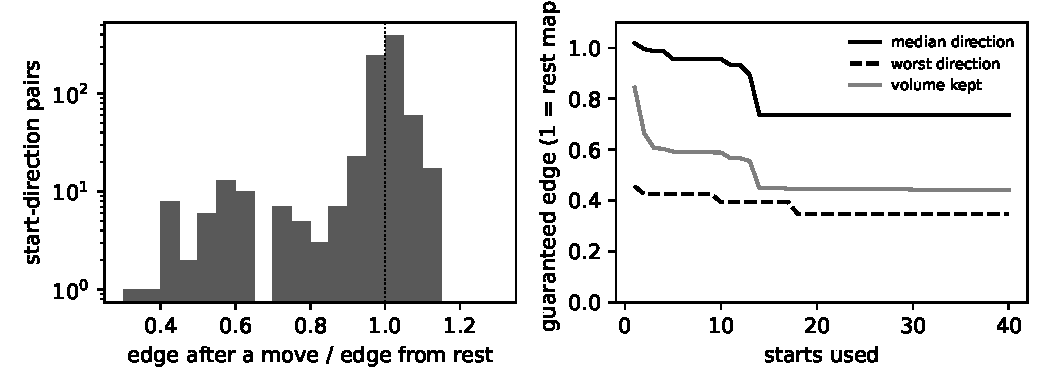
\includegraphics[width=0.9\linewidth]{../figs/fig_wide.pdf}
\caption{Left: edge after one move, as a fraction of the edge from rest, 800 start and direction pairs. Most are
at 1, a tail collapses. Right: the edge that holds from every start used so far, against the number of starts.
Scripted runs.}\label{fig:wide}
\end{figure}

\subsection{Two explanations that failed}
\emph{Leftover tilt.} The tilt is counted from rest, so a move that leaves tilt behind has less budget for the
next one. If that were the cause, the right map would be the rest map with the budget corrected. We repeated the
search with the leftover tilt forgiven. The edge did not go back: the median distance to the rest edge was 0.05
with tilt forgiven against 0.03 with it kept. Tilt is a vector and the budget is a ball around the rest
attitude, so leftover tilt moves the edge outward in some directions and inward in others. % D38

\emph{Enclosed area.} For a free-floating system the attitude change over a closed path grows with the area the
path encloses. Large shifts do only happen at large area (worst $-0.29$~m above 0.09~m$^2$, $-0.05$~m below
0.03~m$^2$), but a linear fit on signed area explains 7\% of the shift. % D38

We do not have a formula for the edge. What we have is the simulation.

\section{Three things to show instead}
\subsection{A map that held from every start}
Take, for each direction, the worst edge over all starts. After 40 starts the median direction keeps 0.74 of the
rest edge and the worst keeps 0.35, which is 44\% of the rest reach by volume. The figure was the same at 20
starts as at 40 (Fig.~\ref{fig:wide}, right), so for starts one move from rest it has probably stopped
shrinking. % D39
It is not a guarantee, and a second move shows it. From 40 starts two moves away from rest, one had already
spent the budget on the way. From 24 of the other 39 the rehearsal refused at least one tip of this map, 4.3\% of
all pairs, on 70 of the 98 directions. Pulling every direction in to 0.8 of its length leaves 11 starts and
0.9\% of pairs. A fixed map cannot be made safe by shrinking it against sampled starts. % D43, data/twoleg*_medium.npz
Measured again on the 98 directions of the map itself, same 40 starts, the map that held keeps 0.67 of the
rest edge on the median direction, 0.24 on the worst, and 40\% of the volume. 28 of the 98 directions keep
less than half and 5 keep everything. % D41, data/wide98_medium.npz

\subsection{A map from where the arm is}
Run the 98 probes again from the current state. On one thread this takes 85 s. Shared over 10 processes it takes
12.6 s from rest and 7.4 s after a 0.3 m move, and 12 processes are no faster. % D39
So this map is right, for a hand that has stopped, and 12 to 13 s old. The tool shows a yellow marker on the hand
while the map is old and a green one when it is current.

\subsection{No map}
Draw nothing. Rehearse every command and refuse the ones that would break the budget. This is never wrong and
gives the operator nothing to plan with: they find the edge by being refused.

\section{Study}
\subsection{Design}
Within subject, four conditions: the rest map (the control), the map that held, the map from the current state,
and no map. 20 participants, balanced Latin square over four orders, five per order.
Goals come in pairs. The first is easy and moves the arm off rest, and is not scored. The second is the test and
starts from where the first left the arm. Whether a goal can be reached is rehearsed from the arm's real state
when it appears. A participant either puts the hand on the goal or gives it up as out of reach, at a cost of 30 s.

Measures, on the second goal of each pair: seconds per goal with the penalty and the rehearsal time in it
(primary), commands the fence had to bring back, reachable goals given up, unreachable goals given up, worst
tilt, and after each block raw NASA-TLX~\cite{hart1988} and one trust rating from 1 to 7.

Hypotheses, written before data: the rest map has the most commands brought back (H1); the map that held has
none and the most reachable goals given up (H2); the current-state map is the fastest per goal (H3); no map has
no commands brought back but is slower and rated as more work (H4). Friedman test over conditions on the
primary measure, Wilcoxon pairs with Holm correction.

\subsection{Results}
\todo{No participant has been run. Ethics approval and consent to settle first. A scripted operator will be run
through all blocks before people are, to see whether seven scored goals per block can separate the conditions
at all; that run will be reported as scripted, not as data.}

\section{Limits}
Simulation only. One arm, one bus mass, one budget. The map that held is tested on one-move starts. The delay of
the current-state map is the delay on one laptop. The reach is probed on 98 lines from one point, so the map is a
set of lines and not a volume with a proof behind it. No contact, no flexible parts, no sensor noise.

\begin{thebibliography}{99}
\bibitem{umetani1989} Y. Umetani and K. Yoshida, ``Resolved motion rate control of space manipulators with generalized Jacobian matrix,'' \emph{IEEE Trans. Robot. Autom.}, vol. 5, no. 3, 1989.
\bibitem{dubowsky1993} S. Dubowsky and E. Papadopoulos, ``The kinematics, dynamics, and control of free-flying and free-floating space robotic systems,'' \emph{IEEE Trans. Robot. Autom.}, vol. 9, no. 5, 1993.
\bibitem{papadopoulos1993} E. Papadopoulos and S. Dubowsky, ``Dynamic singularities in free-floating space manipulators,'' \emph{ASME J. Dyn. Syst. Meas. Control}, vol. 115, 1993.
\bibitem{vafa1990} Z. Vafa and S. Dubowsky, ``The kinematics and dynamics of space manipulators: the virtual manipulator approach,'' \emph{Int. J. Robot. Res.}, vol. 9, no. 4, 1990.
\bibitem{torres1992} M. A. Torres and S. Dubowsky, ``Minimizing spacecraft attitude disturbances in space manipulator systems,'' \emph{J. Guid. Control Dyn.}, vol. 15, no. 4, 1992.
\bibitem{nenchev1999} D. N. Nenchev, K. Yoshida, P. Vichitkulsawat, and M. Uchiyama, ``Reaction null-space control of flexible structure mounted manipulator systems,'' \emph{IEEE Trans. Robot. Autom.}, vol. 15, no. 6, 1999.
\bibitem{yoshida2001} K. Yoshida, K. Hashizume, and S. Abiko, ``Zero reaction maneuver: flight validation with ETS-VII space robot and extension to kinematically redundant arm,'' in \emph{Proc. IEEE ICRA}, 2001.
\bibitem{rosenberg1993} L. B. Rosenberg, ``Virtual fixtures: perceptual tools for telerobotic manipulation,'' in \emph{Proc. IEEE Virtual Reality Annu. Int. Symp.}, 1993.
\bibitem{abbott2007} J. J. Abbott, P. Marayong, and A. M. Okamura, ``Haptic virtual fixtures for robot-assisted manipulation,'' in \emph{Robotics Research}, Springer, 2007.
\bibitem{todorov2012} E. Todorov, T. Erez, and Y. Tassa, ``MuJoCo: a physics engine for model-based control,'' in \emph{Proc. IEEE/RSJ IROS}, 2012.
\bibitem{hart1988} S. G. Hart and L. E. Staveland, ``Development of NASA-TLX: results of empirical and theoretical research,'' in \emph{Human Mental Workload}, 1988.
\end{thebibliography}
\todo{check every reference against the paper itself before submission: volume, issue, pages}
\end{document}
